\section{Indoor Mapping}
The case study used throughout this thesis is the need for indoor geolocalization and routing inside a hospital muiltifloor environment. In this chapter the needed actions to implement the usage of Cisco CMX inside an android application are discussed. Firstly, the mapping component, being MapWize, is discussed, followed by the part of indoor location tracking and an indoor location framework provided by IndoorLocation. Finally the implementation is concluded with the advantages and disadvantages of using the android platform to develop an indoor location application.
\subsection{MapWize}
MapWize is a company that allows developers of an indoor location application to translate architectural floor plans into a digital mapping. Not only do they convert the existing plans but also implement routing and specific points of interest. This eliminates the need for a specific developer team of the company or agency that implements this systems as this is part of the service MapWize provides.
\subsection{MapWize Competitors}
\subsubsection{MazeMap}
MazeMap offers a digital platform to create and editor architectural maps. One of their biggest advantages is the fact that they can incorporate changes in their digital maps based on  a .DWG or .DXF file, which is the used file format for \acrfull{cad} applications \cite{Coon2015}. Other than that it offers positioning and wayfinding by integrating the Cisco \acrlong{cmx} technology. Moreover, MazeMap provides an \acrshort{api} to integrate legacy software or other applications, such as Outlook Exchange, into the ecosystem of indoor location \cite{MazeMapb} \cite{MazeMapa}.
\subparagraph{Case study of Bergen University College}
One of the case studies performed by Cisco is the implementation of Cisco CMX inside the Bergen \acrshort{uc}. The goal of implementing Cisco CMX was to provide students with a \acrfull{byod} policy by creating an 802.11ac WLAN that was scalable to provide each student with Internet access. As stated in the case study, the following devices were used \cite{Magrane2016}:
\begin{itemize}
\item Cisco Aironet 3702e and 3702i \acrlong{ap}s;
\item Cisco 5760 WLAN controllers;
\item Cisco 3850 and 4500-X Series switches;
\item Cisco Catalyst 6500 Series switches;
\end{itemize}
To enable students to use the wayfinding feature, Cisco partnered with MazeMap to create the service and keep it up-to-date with changes in the campus. The major benefit, as mentioned in the case study, is the elimination of crowded hallways that in its turn resulted in a higher, overall happiness amongst students of this \acrlong{uc}.
\begin{figure}[h!]
\centering
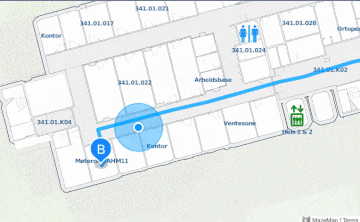
\includegraphics[scale=1]{mazemap_wayfinding}
\caption{Routing feature of MazeMap ~\cite{MazeMapa}}
\label{fig:ips_topologies}
\end{figure}
\begin{figure}[h!]
\centering
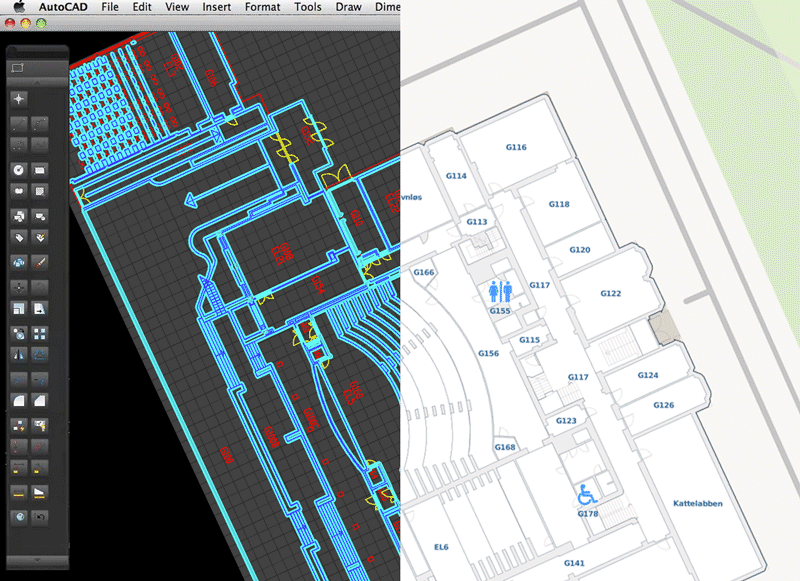
\includegraphics[scale=0.5]{mazemap_mapping}
\caption{Translating floor plans into an interactive map for MazeMap ~\cite{MazeMap}}
\label{fig:ips_topologies}
\end{figure}
\subsubsection{Google Indoor Maps}
\subsubsection{Competitor Analysis}
An overview of the metrics used to compare competitors:
\begin{enumerate}
\item Ability to read and create digital floor plans from \acrshort{cad} files;
\item Interactive editor to edit digital maps;
\item Wayfinding functionality to declare a \acrlong{poi} and determine routes.
\item Position of the \acrlong{mu} shown on the map;
\item If the company creates the interactive maps itself or if the team of developers need to create it.
\item Customizability of the color scheme and icons;
\item Automation: the degree in which changes and modifications to the architectural structure of the environment translates automatically in a changed digital map.
\item Developer support by providing an \acrshort{api} or \acrshort{sdk};
\item Usability;
\item Additional Features;
\end{enumerate}
One thing to be noticed is that the cost is not used as a metric as most of the competitors - apart from MapWize - work with a quote-only pricing.


TABLE

\subsection{MapWize SDK for Android Applications}
\subsubsection{Application Setup}
\section{Indoor Location tracking}
\subsection{IndoorLocation Framework}
\subsubsection{Application Setup}
\subsection{Applying IndoorLocation Framework to Android Applications}
\section{Conclusion}
